\chapter{Problema 2: Identificação de Indivíduos}
\label{chap:ident_individuos}

\section{Introdução}
\label{chap4:sec:intro}
O reconhecimento facial de indivíduos, face a um \textit{dataset} conhecido, configurou o segundo desafio proposto. Foi usado o \textit{dataset} AR \cite{ar_site}, que contém 134 pessoas e mais de 3000 imagens (todas as pessoas têm imagens com diferente iluminação, expressões distintas ou adereços físicos). Alguns indivíduos registaram, ainda, imagens em dois dias diferentes (as mesmas variações acima mencionadas, mas registadas em dias distintos).


\noindent A figura \ref{fig:ar_dataset} apresenta as imagens recolhidas de um indivíduo, a título de exemplo.

\begin{figure}[h]
\centering
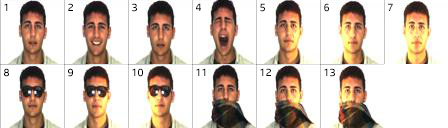
\includegraphics[width=380pt]{ar_dataset.png}
\caption{Exemplos de imagens do \textit{dataset} AR.}
\label{fig:ar_dataset}
\end{figure}
\newline
\noindent
\newline
\noindent
\newline
\noindent
\section{Pré-processamento dos dados}
\label{chap3:sec:metodo}
Ao contrário do processo descrito no capítulo anterior, as imagens deste \textit{dataset} já têm todas o mesmo tamanho e não existe necessidade de avaliar o tipo de movimento. Assim, apenas é necessário separá-las por indivíduo, gerar instâncias erradas para cada positiva e gerar o ficheiro CSV final (figura \ref{fig:processo2}).

\begin{figure}[h]
\centering

\includegraphics[width=380pt]{pipeline2.png}
\caption{\textit{Pipeline} de pré-processamento.}
\label{fig:processo2}
\end{figure}

\subsection{Separação das sequências}
\label{chap4:subsec:separacao}
Todas as imagens foram agrupadas de acordo com o indivíduo a que pertencem, sendo estes posteriormente divididos em conjuntos de treino, validação e teste (com a seguinte distribuição: 80\%, 10\% e 10\%).

\subsection{Geração de sequências erradas}
\label{chap4:subsec:erradas}

Foram exploradas duas formas de combinar as imagens dos indivíduos:

\begin{enumerate}
    \item \textbf{Sequências de duas imagens:} uma sequência certa será composta por duas imagens do mesmo indivíduo. Independentemente das caraterísticas específicas das imagens, se a pessoa for a mesma, a sequência é válida. \newline
    \noindent Para gerar sequências erradas, parte-se da sequência certa correspondente e é sorteado um outro indivíduo do mesmo conjunto (treino, validação ou teste) e uma das duas imagens, que se vai trocar pela equivalente do indivíduo sorteado. Por exemplo, se uma instância positiva tiver uma imagem em que o indíviduo sorri e outra em que está de óculos de sol, e for sorteada a dos óculos de sol, esta será substituída na instância errada pela imagem do indivíduo sorteado na qual também tem óculos de sol (figura \ref{fig:trocas2}).

    \begin{figure}[h]
      \centering
      \begin{subfigure}{3.6cm}
        \centering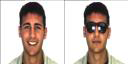
\includegraphics[width=3.6cm]{seq_certa.png}
        \caption{}
      \end{subfigure}
      \hspace{1em}
      \begin{subfigure}{3.6cm}
        \centering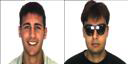
\includegraphics[width=3.6cm]{seq_errada.png}
        \caption{}
      \end{subfigure}
      \caption{Sequência de duas imagens válida (a) e inválida (b).}
      \label{fig:trocas2}
    \end{figure}
    
    \item \textbf{Sequências de três imagens:} uma sequência certa será composta por duas imagens do mesmo indivíduo e uma imagem de outro indivíduo do mesmo conjunto. Deste modo, é possível obter mais combinações, não só para a aprendizagem mas também para a futura identificação de imagens nunca vistas.\newline
    \noindent Uma instância negativa consiste em manter duas imagens da positiva (uma das duas imagens do mesmo indivíduo e a do indivíduo diferente) e trocar a restante por uma equivalente (figura \ref{fig:trocas3}).
    
    \begin{figure}[h]
      \centering
      \begin{subfigure}{5.3cm}
        \centering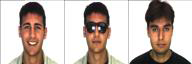
\includegraphics[width=5.3cm]{sequencia_3_boa.png}
        \caption{}
      \end{subfigure}
      \hspace{1em}
      \begin{subfigure}{5.3cm}
        \centering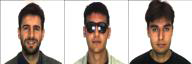
\includegraphics[width=5.3cm]{sequencia_3_ma.png}
        \caption{}
      \end{subfigure}
      \caption{Sequência de três imagens válida (a) e inválida (b).}
      \label{fig:trocas3}
    \end{figure}
    
\end{enumerate}

\noindent Os conjuntos de imagens válidos e inválidos foram colocados num ficheiro .csv, necessário para a aprendizagem por parte da \ac{CNN}.

\section{Fase de aprendizagem}
\label{chap4:sec:aprendizagem}
A aprendizagem decorreu de acordo com os parâmetros e configurações descritos na tabela \ref{tab:aprendizagem_ar}, que contém também a taxa de acerto no conjunto de teste (os resultados são semelhantes nesta fase, quer seja com sequências de duas ou três imagens).

\begin{table}[h]
\centering
\begin{tabular}{|l|r|}
\hline
\textbf{Parâmetro} & \textbf{Valor}\\
\hline
\hline
Épocas & 65  \\
\hline
Probabilidade de \textit{dropout} & 1.0  \\
\hline
Tamanho de \textit{batch} & 100  \\
\hline
Sequências & $\sim75000$  \\
\hline
\hline
\textbf{Acerto (conj. teste)} & \textbf{82\%-83\%}\\
\hline
\end{tabular}
\caption{Parâmetros e configurações na aprendizagem.}
\label{tab:aprendizagem_ar}
\end{table}

\begin{figure}[h]
\centering
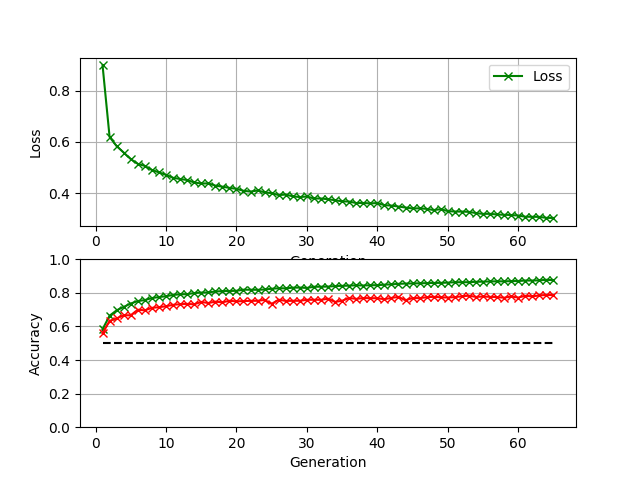
\includegraphics[width=300pt]{aprendizagem_ar.png}
\caption{Aprendizagem da \ac{CNN} sobre o \textit{dataset} AR.}
\label{fig:aprendizagem_dataset}
\end{figure}

\newline
\noindent
\newline
\noindent

\section{Discussão e Resultados}
\label{chap4:sec:final}
Foram desenvolvidos dois programas, usando os dois modelos treinados ora com duas sequências (chamado Face\_match1) ora com três (Face\_match2), cujo objetivo seria tomar como \textit{input} uma imagem nunca antes vista (colocada numa pasta específica) e retornar um ranking dos indivíduos com maiores chances de serem o indivíduo presente na foto de entrada.\newline
\noindent A título experimental, foi retirada, de cada pessoa, a imagem em que está zangada. Todas estas imagens foram então colocadas numa pasta própria e qualquer uma delas pode ser usada para testar o sistema desenvolvido. \newline

\noindent Para testar os dois sistemas desenvolvidos, foi usada uma galeria de imagens conhecidas pela rede (neste caso, as imagens de cada indivíduo com expressão neutra). 

\begin{figure}[h]
\centering
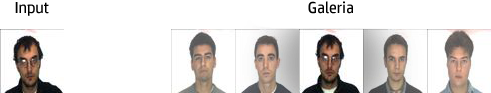
\includegraphics[width=350pt]{exemplo.png}
\caption{Objetivo dos sistemas desenvolvidos.}
\label{fig:exemplo}
\end{figure} 
\newline
\noindent A figura \ref{fig:face_match_rankings} apresenta algumas observações retiradas das experiências realizadas com as imagens passíveis de ser testadas (134 imagens com expressão zangada). 
\begin{figure}[H]
  \begin{subfigure}{15.0cm}
    \centering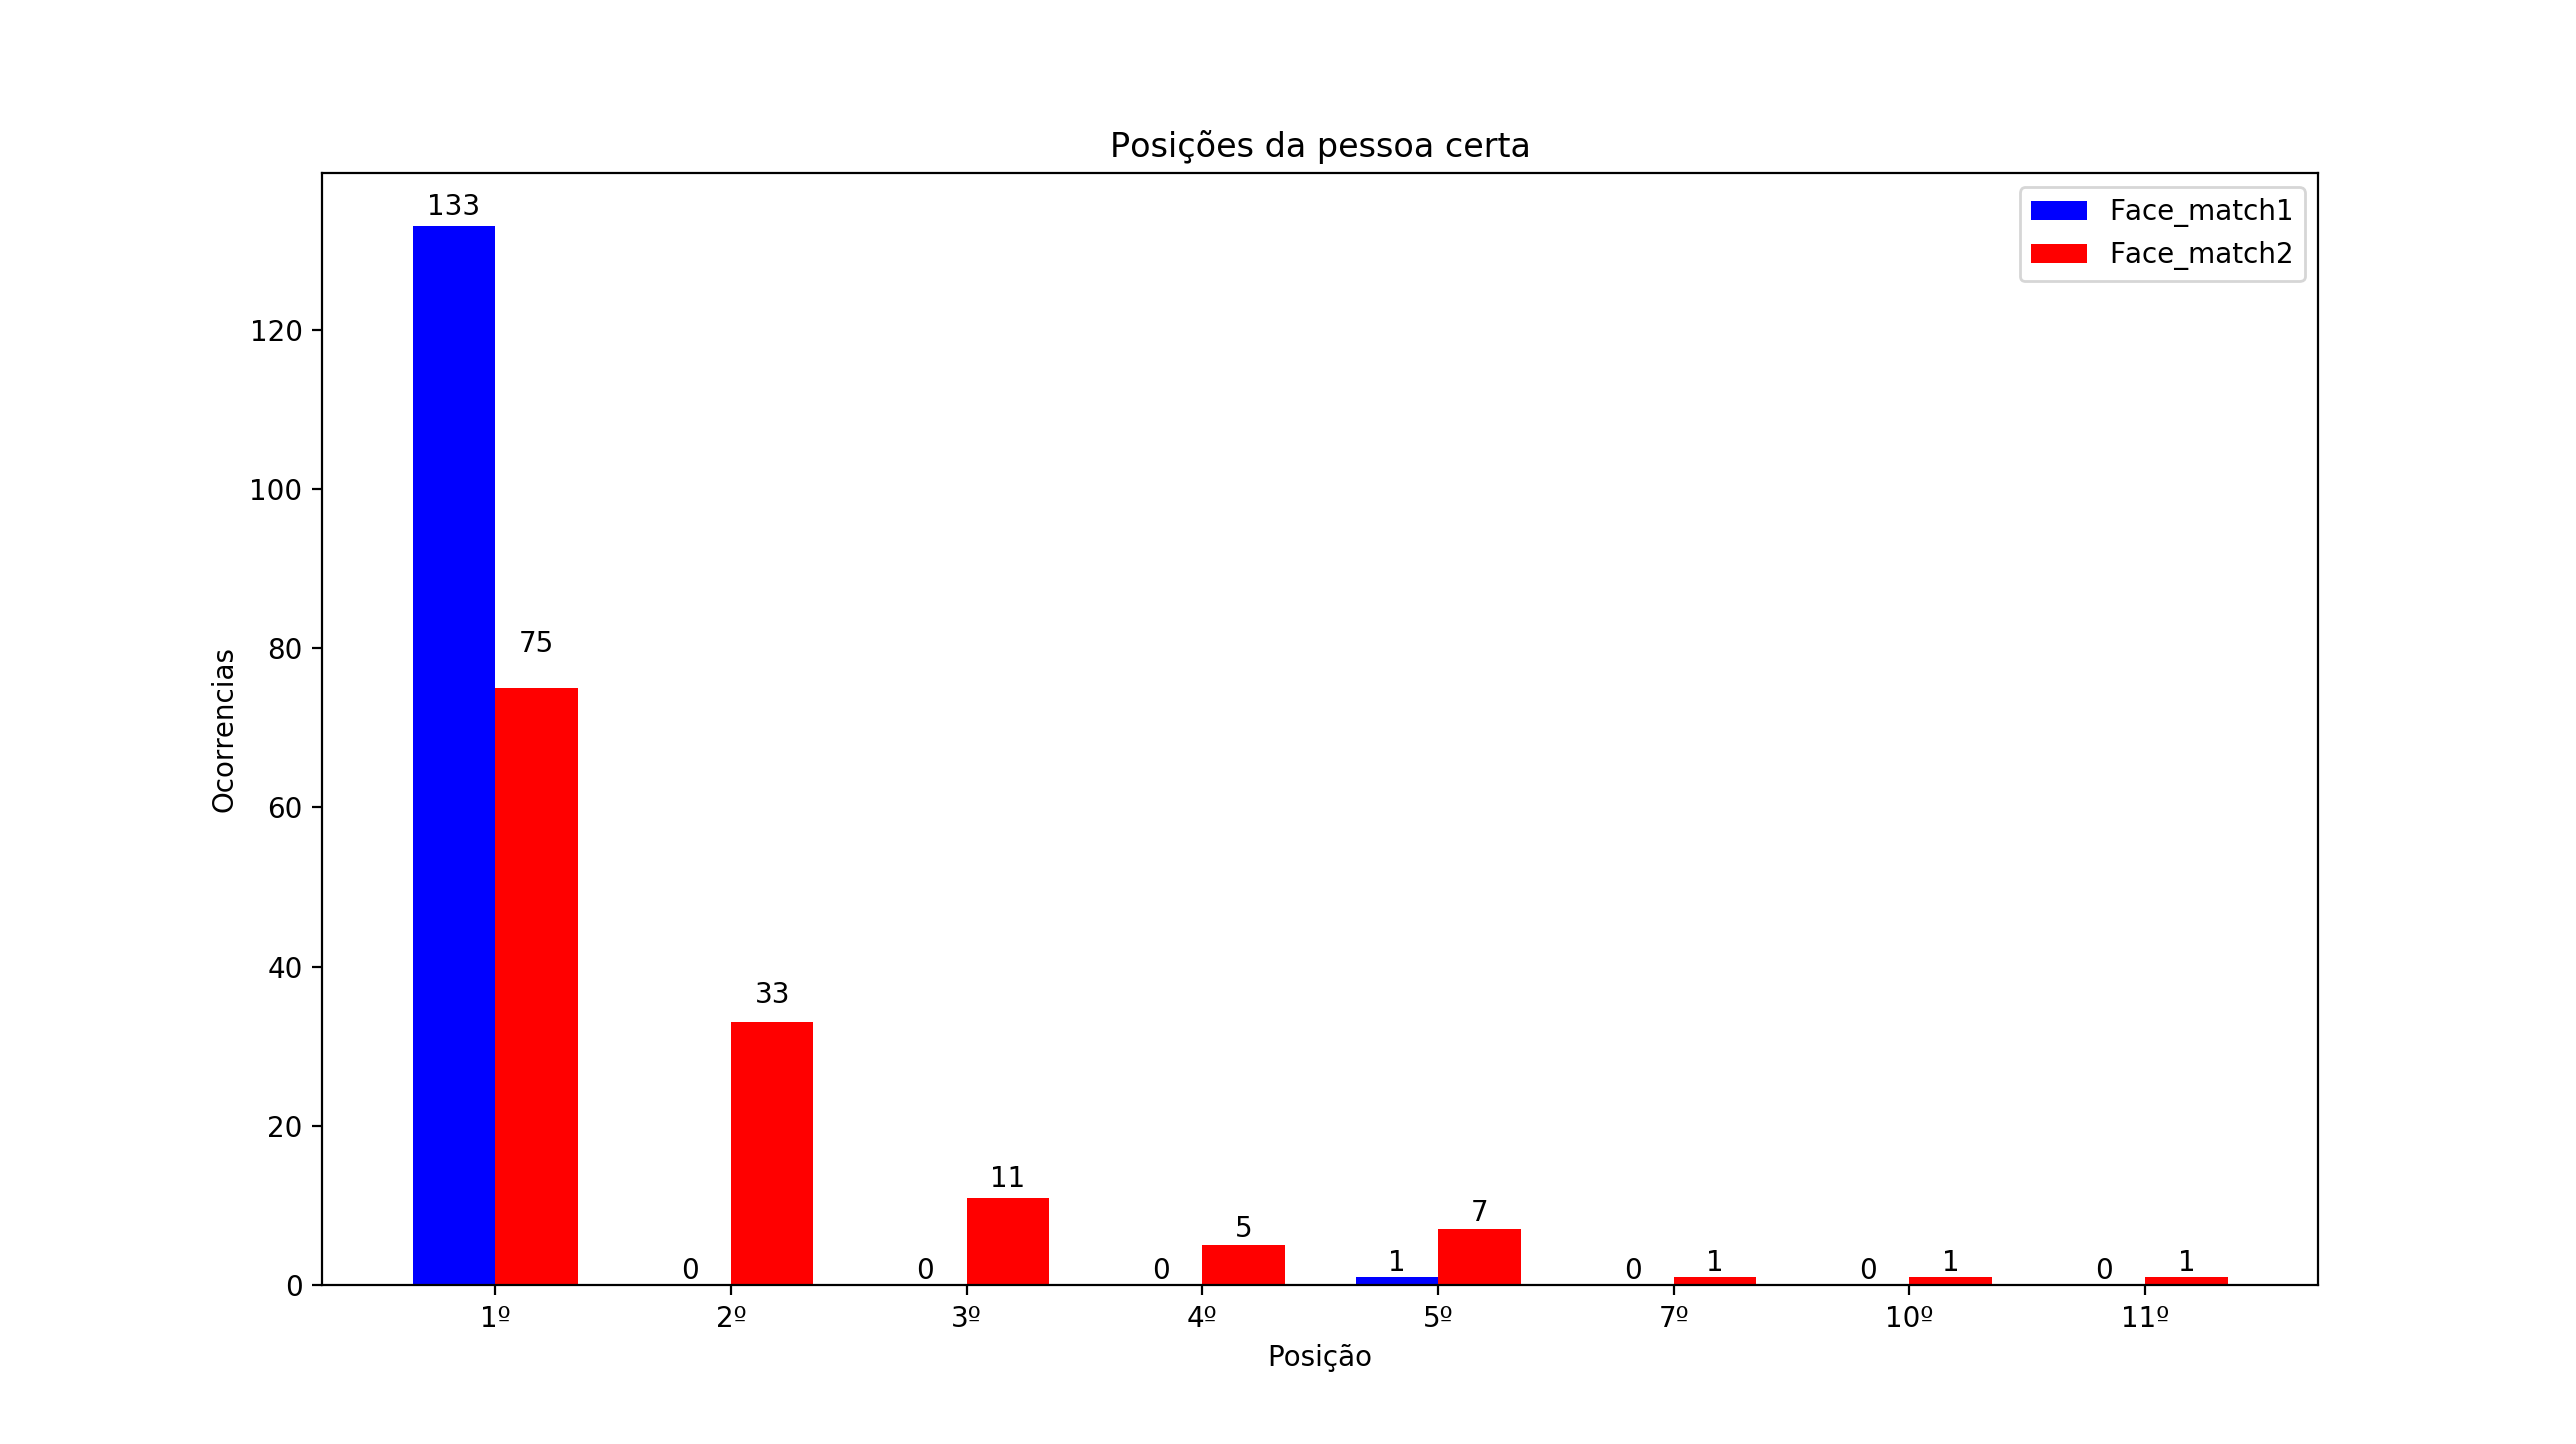
\includegraphics[width=15.0cm]{face_match_rankings.png}
    \caption{}
  \end{subfigure}
  \begin{subfigure}{15.0cm}
    \centering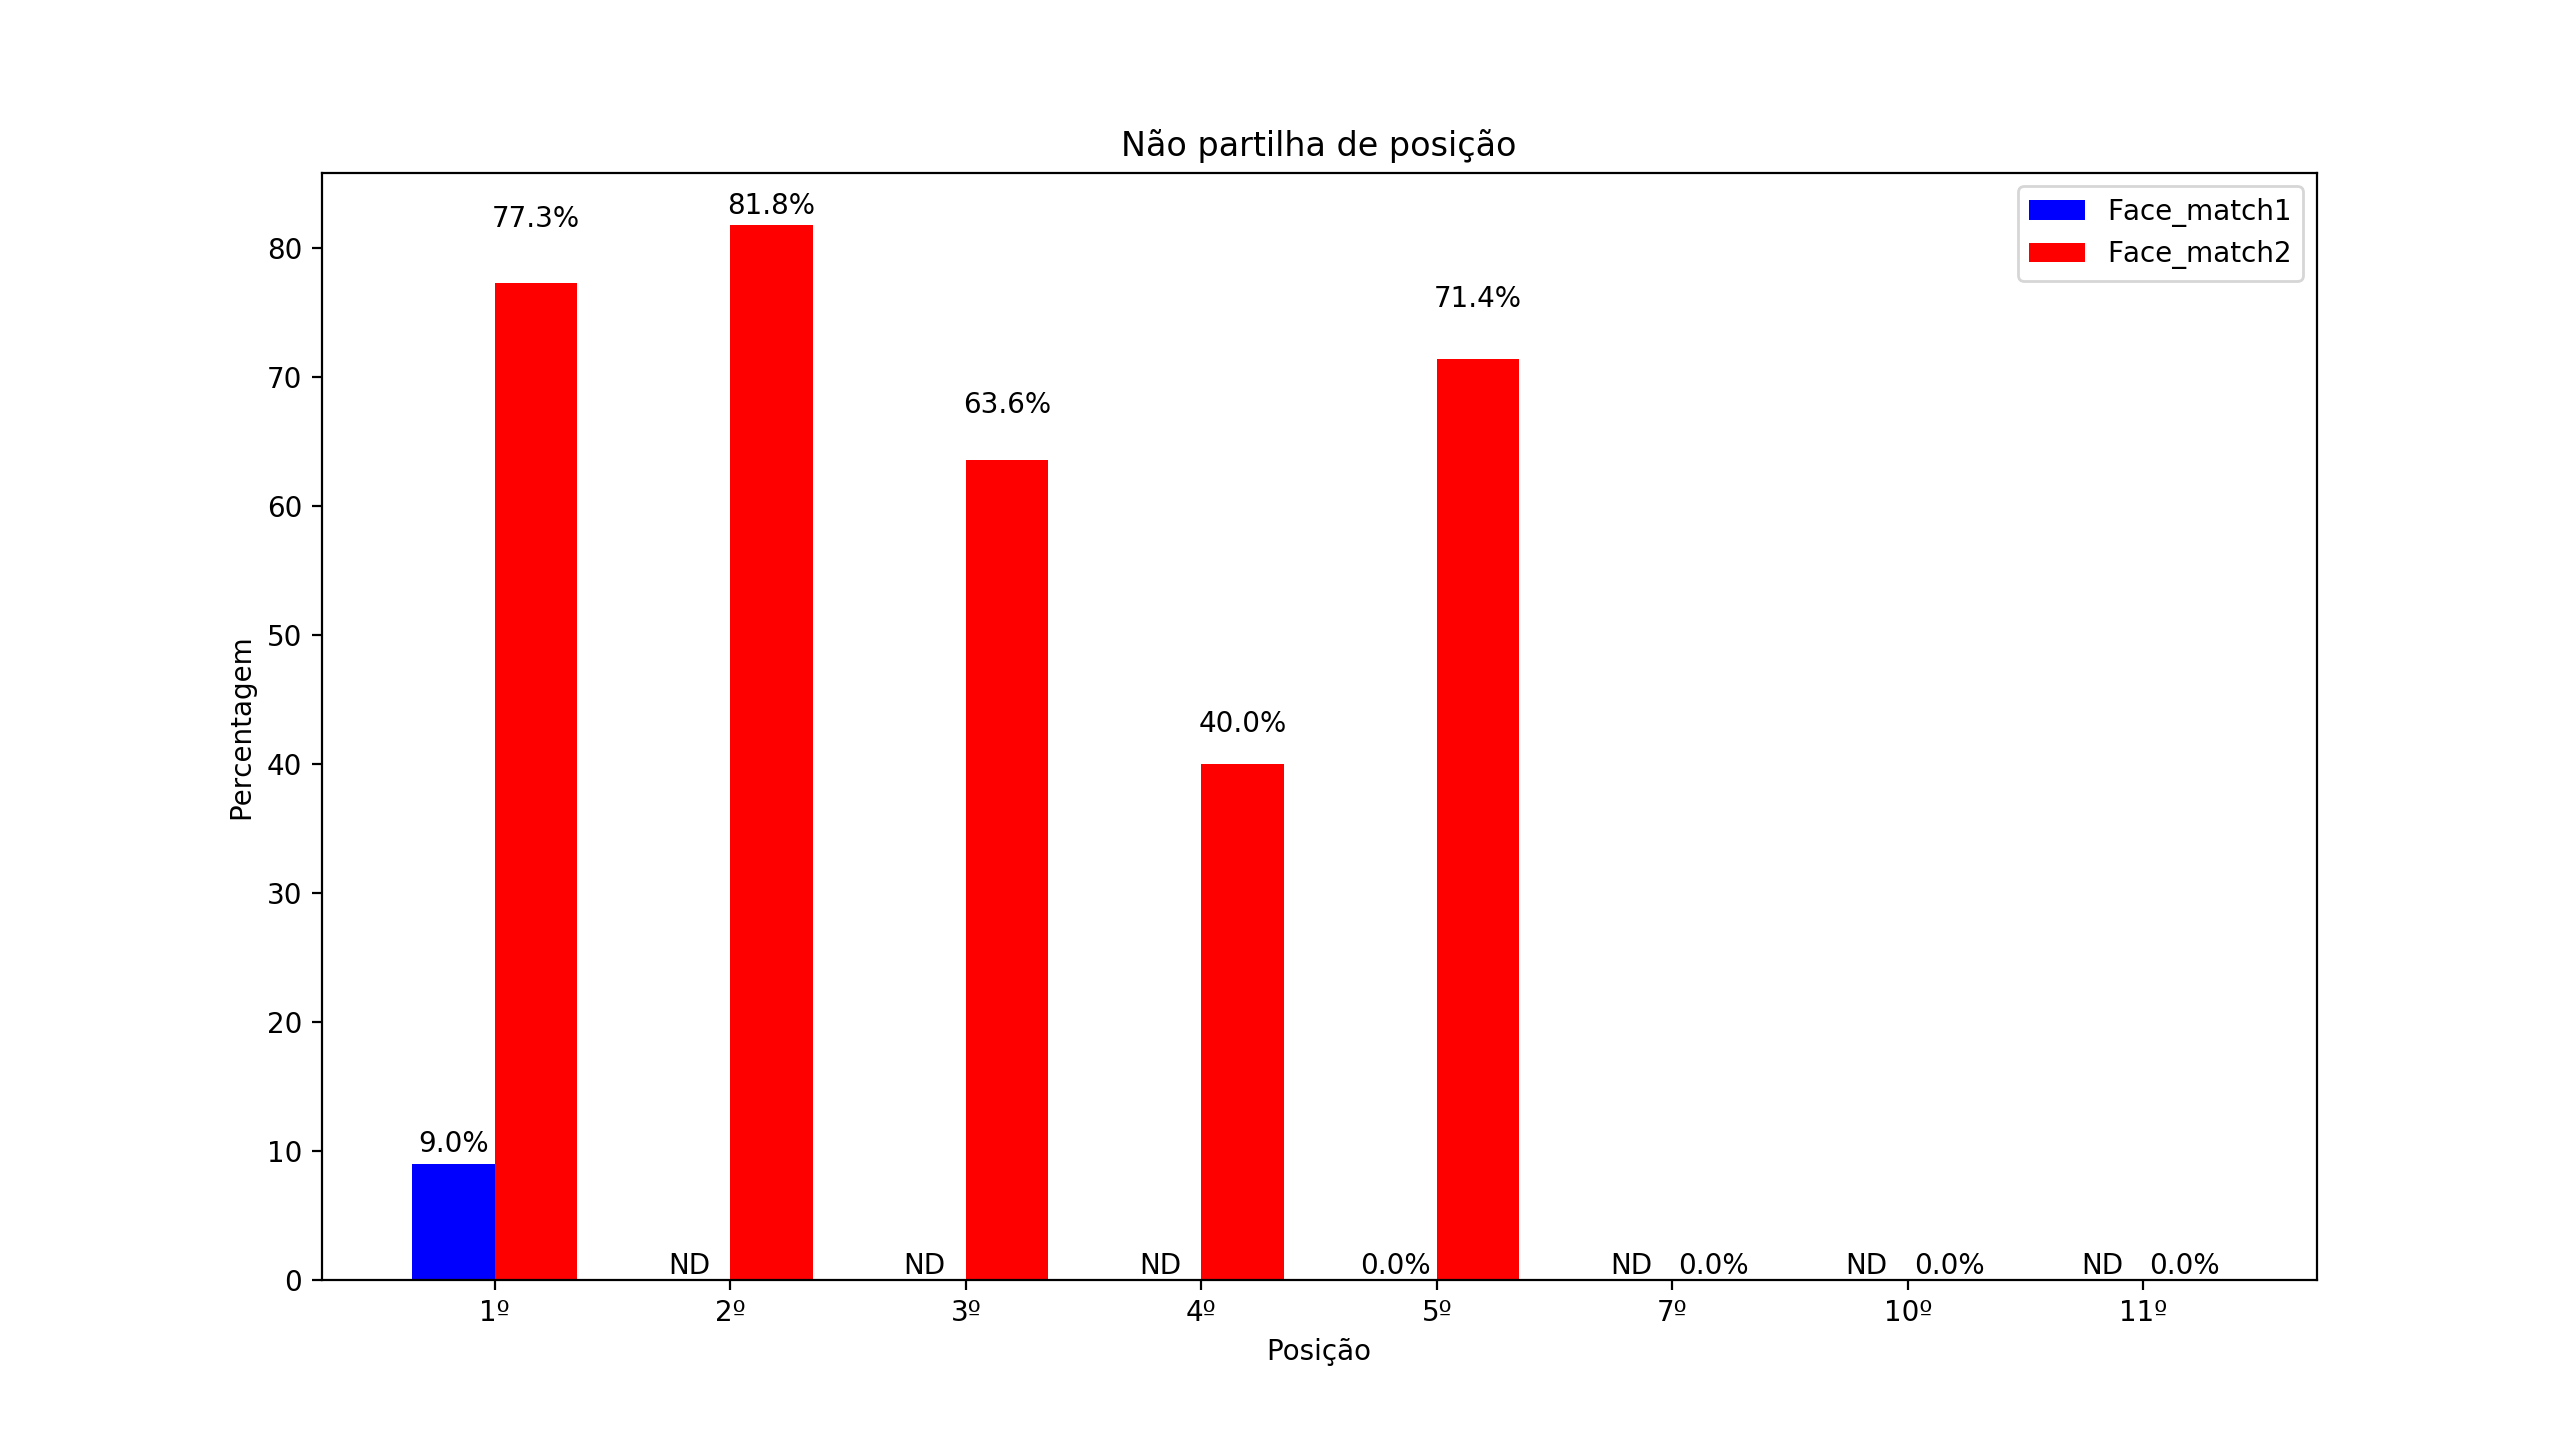
\includegraphics[width=15.0cm]{face_match_rankings2.png}
    \caption{}
  \end{subfigure}
  \caption{Acertos de cada solução (a) e a taxa de partilha de posições (b).}
  \label{fig:face_match_rankings}
\end{figure}

\newline
\noindent
\noindent Pela análise dos gráficos, é possível perceber que a solução que conjuga apenas duas imagens (Face\_match1) coloca o indivíduo certo na 1ª posição com maior frequência. Contudo, coloca também outros indivíduos, não sendo por isso a mais determinista.\newline
\noindent Por outro lado, a solução que opera sobre três imagens em simultâneo (Face\_match2), é menos certeira nas avaliações que faz, mas não apresenta o problema de colocar demasiadas pessoas numa mesma posição. \newline
\noindent De um modo geral, os casos em que a rede falhou prendem-se com os exemplos retratados na figura \ref{fig:falhas}. Quando o mesmo indivíduo possui imagens muitos distintas, é dada uma resposta negativa falsa. Por outro lado, quando são duas pessoas diferentes, mas parecidas, é dada uma resposta positiva falsa.

\begin{figure}[h]
  \centering
  \begin{subfigure}{4.5cm}
    \centering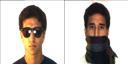
\includegraphics[width=4.5cm]{ar_falha1.jpg}
    \caption{}
  \end{subfigure}
  \hspace{1em}
  \begin{subfigure}{6.8cm}
    \centering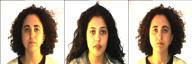
\includegraphics[width=6.8cm]{ar_falha2.jpg}
    \caption{}
  \end{subfigure}
  \caption{Casos típicos de falha.}
  \label{fig:falhas}
\end{figure}